\documentclass{article}
\usepackage[utf8]{inputenc}
\usepackage{graphicx}

\title{Teori}
\author{itsmekil707}
\date{October 2019}

\begin{document}
\title{Teori}
\author{Akil Munawwar \\ 1184041 \\ D4 TI 1B}

\maketitle

\part{Variabel}
\section{Cara Pemakaian Variabel}
\begin{figure}[!htbp]
    \centering
    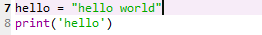
\includegraphics[scale=1]{Variabel.PNG}
    \caption{Contoh Variabel}
\end{figure}
Disini terdapat variabel "hello". Sebelum itu pada penulisan variabel tidak boleh memakai angka di depan, tidak boleh menggunakan spasi, jika ingin melanjutkan dua kata maka menggunakan \textit{underscore}. Selanjutnya pada figure1, terdapat nama variabel hello dengan nilai "hello world".
\newpage

\section{Input dan Output}
Pada figure2, terdapat kodingan yang dibutuhkan untuk input user. Nantinya jika kita run, maka akan muncul perintah input untuk user.
\begin{figure}[!htbp]
    \centering
    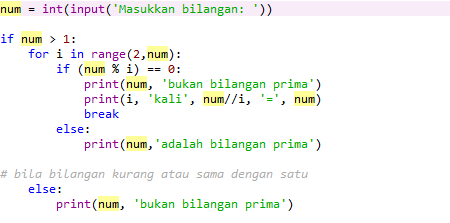
\includegraphics[scale=1]{Inputan.PNG}
    \caption{Kodingan untuk Inputan User}
\end{figure}
\paragraph{}
Nantinya setelah di run, ada perintah input dari user. Misal kita input angka 2, maka akan muncul output berupa "2 bukan bilangan prima". Seperti pada figure3
\begin{figure}[!htbp]
    \centering
    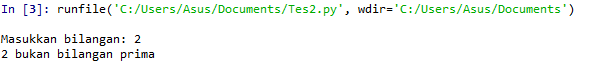
\includegraphics[scale=0.4]{Output.PNG}
    \caption{Output ke Layar}
\end{figure}
\newpage
\section{Aritmatika}
Operasi aritmatika pada python terdiri dari pertambahan, perkalian, pengurangan dan pembagian. Ketika ingin melakukan operasi aritmatika, tentukan dulu variabel yang akan dibuat. Misal a = 2 dan b = 3. Maka dibawahnya dibuat lagi variabel C untuk menjumlahkan kedua variabel diatas tadi.
\begin{figure}[!htbp]
    \centering
    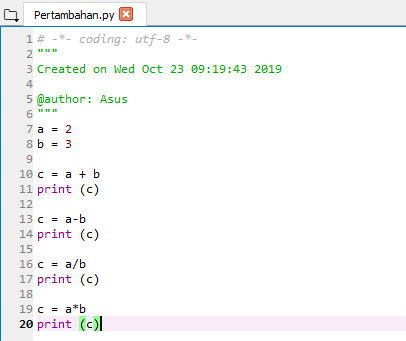
\includegraphics[scale=1]{Aritmatika.PNG}
    \caption{Kodingan Aritmatika}
\end{figure}
\paragraph{}
Setelah itu, kita run dan hasilnya akan seperti figure5
\begin{figure}[!htbp]
    \centering
    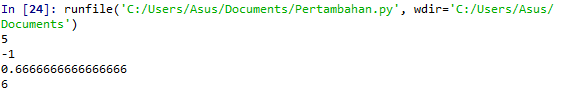
\includegraphics[scale=0.7]{OutputAritmatika.PNG}
    \caption{OutputAritmatika}
\end{figure}
\newpage
\section{Konversi Int ke Str}
Cara Konversi nya ialah dengan menentukan variabel. Variabel A menampung tipe data Integer dengan nilai 100. Setelah itu kita tentukan variabel string. Sesudah itu, kita panggil variabel string dengan perintah print.
\begin{figure}[!htbp]
    \centering
    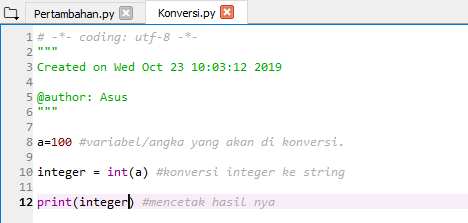
\includegraphics[scale=0.8]{KonvIntKeStr.PNG}
    \caption{Konversi Int Ke Str}
\end{figure}
\paragraph{}
Hasilnya akan seperti ini.
\begin{figure}[!htbp]
    \centering
    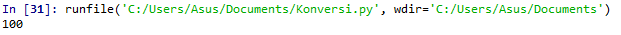
\includegraphics[scale=0.6]{HasilKonvIntKeStr.PNG}
    \caption{Hasil Konversi Str ke Int}
\end{figure}
\newpage
\section{Konversi Str ke Int}
Cara Konversi ini sama seperti konversi yang Integer ke String.
\begin{figure}[!htbp]
    \centering
    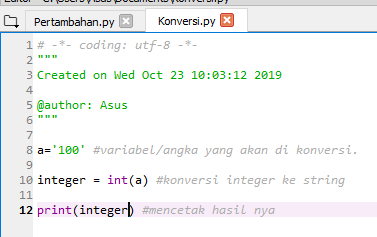
\includegraphics{KonvStrKeInt.PNG}
    \caption{Konversi Str ke Int}
\end{figure}
\paragraph{}
Hasilnya akan seperti ini.
\begin{figure}[!htbp]
    \centering
    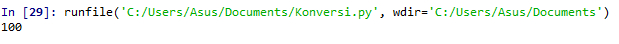
\includegraphics[scale=0.6]{HasilKonvStrKeInt.PNG}
    \caption{Hasil Konversi Str ke Int}
\end{figure}
\newpage
\section{Perulangan For}
Perulangan for akan terjadi selagi nilai i dibawah 10
\begin{figure}[!htbp]
    \centering
    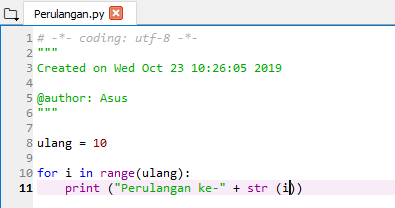
\includegraphics{Perulangan.PNG}
    \caption{Kodingan Perulangan}
\end{figure}
\paragraph{}
Ketika sudah selesai, maka kita run, dan hasilnya akan seperti ini.
\begin{figure}[!htbp]
    \centering
    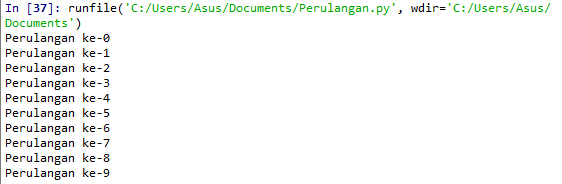
\includegraphics[scale=0.6]{OutputPerulangan.PNG}
    \caption{Output Perulangan}
\end{figure}
\newpage
\section{Perulangan While}
Perulangan while akan terjadi hingga kondisi tersebut true atau tercapai.
\begin{figure}[!htbp]
    \centering
    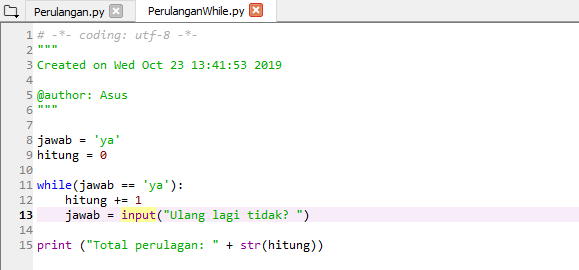
\includegraphics[scale=0.6]{PerulanganWhile.PNG}
    \caption{Kodingan Perulangan While}
\end{figure}
\paragraph{}
Ketika sudah diketik, maka kita run, dan hasilnya seperti ini.
\begin{figure}[!htbp]
    \centering
    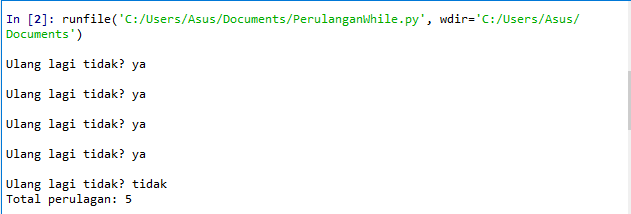
\includegraphics[scale=0.6]{OutputPerulanganWhile.PNG}
    \caption{Output Perulangan}
\end{figure}
\newpage
\section{Kondisi}
Kondisi ialah suatu keadaan dimana ada kondisi True dan False. Contoh nya seperti di figure14.
\begin{figure}[!htbp]
    \centering
    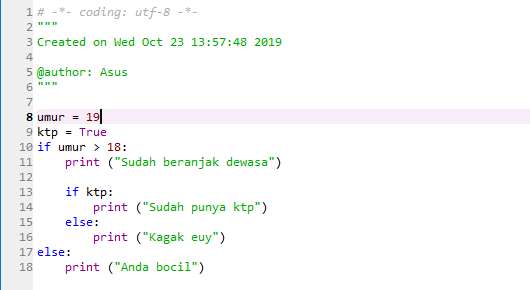
\includegraphics[scale=0.6]{Kondisi.PNG}
    \caption{Kodingan Kondisi}
\end{figure}
\paragraph{}
Kondisi biasanya ditandai dengan \textit{if} dan juga dipakai ketika membuat sistem login. Yang dimana jika kita input user benar namun password salah. Itu akan menampilkan suatu pop up. Tetapi jika kita benar input keduanya maka berhasil login. Dan pada contoh kodingan ini, saya tidak memakai yang login. Tetapi saya memakai kondisi dimana jika umurnya lebih dari 18, maka dia mempunyai KTP.
\begin{figure}[!htbp]
    \centering
    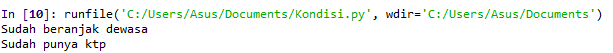
\includegraphics[scale=0.6]{OutputKondisi.PNG}
    \caption{Output Kondisi}
\end{figure}
\newpage
\section{Jenis Error Yang Ditemukan}
Jenis error yang ditemukan sering terlihat pada perintah \textit{print}, errornya karena kurangnya memberi tanda kurung pada setiap perintahnya.
\begin{figure}[!htbp]
    \centering
    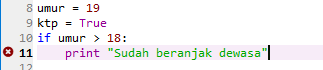
\includegraphics{error.PNG}
    \caption{Error Perintah Print}
\end{figure}
\paragraph{}
Cara mengatasinya tinggal memberi tanda kurung pada perintah print sebagai berikut.
\begin{figure}[!htbp]
    \centering
    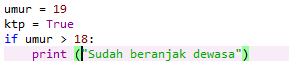
\includegraphics{solusi.PNG}
    \caption{Solusi Error}
\end{figure}
\newpage
\section{Cara Menggunakan Try Except}
Try Except sering digunakan untuk mengatasi error yang ada. Metode ini digunakan biasanya pada operator aritmatika. Contoh seperti dibawah ini.
\begin{figure}[!htbp]
    \centering
    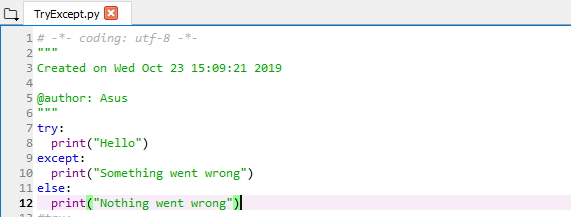
\includegraphics[scale=0.6]{TryExcept.PNG}
    \caption{Kodingan Try Except}
\end{figure}
\paragraph{}
Ketika dijalankan dan tidak ada error, maka selanjutnya dia akan menampilkan yang \textit{nothing went wrong} seperti pada gambar dibawah ini.
\begin{figure}[!htbp]
    \centering
    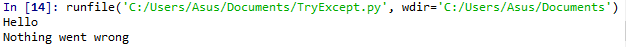
\includegraphics[scale=0.6]{OutputTryExcept.PNG}
    \caption{Output Try Except}
\end{figure}
\end{document}